\chapter{Einleitung}

Sowohl unser Geschäfts- als auch unser Alltagsleben sind heutzutage durch Softwaresysteme geprägt.
Dabei werden sowohl aus Benutzersicht als auch aus technischer Sicht hohe Anforderungen an die
verwendete Software gestellt. Eine Software soll gut bedienbar, zuverlässig, sicher, vernetzbar,
anpassbar und dabei auch möglichst günstig sein. Um diesen Anforderungen gerecht zu werden, werden
die Software Projekte auf technischer Seite zum einen immer komplexer und größer, zum anderen muss
ein solches Projekt häufig über Jahre oder Jahrzehnte hinweg gepflegt und gewartet werden. Im Laufe
dieser Zeit kann es passieren, dass sich gewisse Anforderungen an das Projekt ändern oder dass die
Software auf eine neu entwickelte Technologie übertragen werden soll. Nicht zuletzt spielen auch die
Kosten, die in eine solche Entwicklung einfließen eine entscheidende Rolle. Daher werden immer neu
Methoden benötigt, um die effektive Entwicklung und Wartung eines Softwaresystems zu ermöglichen.

% \begin{quote}
% "`The myth of the standalone application, never needing repair, never needing
% integration, with data models inviolate and secret, died a long and painful death
% through the end of the Twentieth Century. Despite the sure knowledge that every
% application ever built must be built to last, to be integrated, to be updated, most
% software developers ignored these facts and built only to the specification in front of
% them. Assumptions not in evidence–'this application will only be needed for the next
% few years,` [\ldots]"' \cite{MDA} (S.5)
% \end{quote}

% Eine fehlerhafte Annahme, die in der Vergangenheit oft getroffen wurde, ist die, dass eine Software
% nur ein paar Jahre gebraucht wird und anschließend keine Weiterentwicklung und Wartung mehr
% stattfindet. Würden wir unter der gleichen Annahme Gebäude bauen, dann wäre es uns unmöglich diese
% zu verändern oder auch einfach nur umzudekorieren, um sie an neue Gegebenheit anzupassen und im
% schlimmsten Fall würde sie auf Dauer einfach in sich zusammenfallen. Während dies neue Arbeit für
% Bauarbeiter schafft, sind diese Umstände hingegen für die Menschen, die in diesen Gebäuden leben und
% arbeiten absolut inakzeptabel. Deshalb gibt es eigentlich nur sehr wenig Ausreden dafür eine
% Software zu entwickeln, ohne vorher sorgfältige Planungsarbeiten durchzuführen. Die Planungsarbeiten
% helfen nicht nur dabei ein Softwaresystem einfach zu entwickeln, zu integrieren und zu warten,
% sondern sie geben uns auch die Möglichkeit einige Teile des Systems automatisch zu erzeugen. So, als
% ob eine Maschine sofort aus dem Modell eines Architekten die Grundkonstruktion eines Gebäudes
% erstellten könnte. Mehr noch, wenn wir verschiedene Konstruktionen verbinden wollen, können wir
% automatisch Brücken basierend auf den vorliegenden Modellen generieren und wenn ein neuer
% feuerfester Stahltyp entwickelt wurde, dann können wir alle Konstruktionen auf dieser Grundlage
% einfach erneut generieren. \cite{MDA} (S.5-6)

% The myth of the standalone application, never needing repair, never needing
% integration, with data models inviolate and secret, died a long and painful death
% through the end of the Twentieth Century. Despite the sure knowledge that every
% application ever built must be built to last, to be integrated, to be updated, most
% software developers ignored these facts and built only to the specification in front of
% them. Assumptions not in evidence–“this application will only be needed for the next
% few years,” a particular favorite–wreaked havoc in the business world as the clock
% ticked over to the year 2000. Nevertheless, most software continues to be written
% ignoring the realities of constantly shifting infrastructure, constantly changing
% requirements, and most importantly, a new “hot technology” trumpeted on the covers
% of every IT trade journal every 18 months.

% After all, if we built buildings the way we built software, we would be unable to
% connect them, change them or even redecorate them easily to fit new uses; and worse,
% they would constantly be falling down. While this might generate new income for
% construction workers, it might not be acceptable to those who live and work in those
% buildings.

% In fact, we have very little excuse to build software without first doing careful design
% work; design not only leads to systems that are easier to develop, integrate and
% maintain–but also because we have the ability to automate at least some of the
% construction. Imagine if the construction worker could take his blueprint, crank it
% through a machine, and have the foundation of the building simply appear. Not likely
% outside the Jetsons’ world, but an everyday occurrence in the software world. We can
% take models, defined in standards like OMG’s own UML, MOF and CWM, and
% automate the construction of data storage and application foundations. Even better,
% when we need to connect these “buildings” to each other we can automate the
% generation of bridges and translators based on the defining models; and when a new,
% more fire-resistant type of steel is invented, we can regenerate for the new
% infrastructure.

Ein Konzept, welches in der Praxis immer mehr an Bedeutung gewinnt, ist das \textit{Model-Driven
Software Development} (MDSD) \cite{MDA}, \cite{MDSD}, \cite{GPR06}. Die Philosophie hinter diesem
Softwareentwicklungskonzept ist es,
% Eben diese Philosophie steckt hinter dem Softwareentwicklungskonzept des \textit{Model-Driven
% Software Development} (MDSD),
möglichst viele Teile der Softwareherstellung zu automatisieren. Als Grundlage hierfür werden
hinreichend formale und zugleich abstrakte Modelle verwendet, aus denen dann verschiedene Artefakte
des Systems abgeleitet werden. Modelle werden dabei vorzugsweise als Diagramme angelegt, da komplexe
Strukturen visuell so besser überblickt werden können. Die abgeleiteten Artefakte können zum einen
ausführbare Programmteile in einer bestimmten Zielsprache wie z.B. Java oder C\# sein, zum anderen
können aber auch Konfigurationsdateien, Datenbankskripte, Testfälle oder Dokumentationsdateien aus
den Modellen automatisch abgeleitet werden, während  dieser Prozess in der klassischen Software
Entwicklung eine manuelle Tätigkeit ist. Daher nehmen Modelle in MDSD ein zentrale Stellung im
gesamten Entwicklungsprozess einer Software ein. \cite{MDSD} (S.11 - 13)

\begin{quote}
"`Das bedeutet auch, dass Modelle und einzelne Modellelemente z.B. bezüglich Versionierung genauso
zu behandeln sind wie Quelltext. Verteilte Teams müssen also in der Lage sein, Modelle aus einem
Versionsverwaltungssystem auszuchecken, einzelne Modellelemente zu bearbeiten, mit früheren
Versionen zu vergleichen, konkurrierende Modifikationen aufzulösen und den neuen Stand wieder in das
Versionsverwaltungssystem einzuchecken."' \cite{MDSD} (S.12)
\end{quote}

Um verschiedene Versionen von Modellen zu vergleichen und um die Unterschiede zwischen den Versionen
anzuzeigen, werden s.g. Differenzwerkzeuge benötigt. Differenzwerkzeuge, mit denen normalerweise
Quelltexte verglichen werden, sind für strukturierte Modelle nicht zu gebrauchen \cite{LE09}, da
diese auf Basis ihrer Graphrepräsentation verglichen werden müssen. Viele verfügbare
Differenzwerkzeuge arbeiten generisch, so dass sie für verschiedene Modelltypen eingesetzt werden
können. Ein Nachteil, der daraus resultiert, ist, dass die Modelle anhand ihrer internen
Repräsentation verglichen werden müssen. Diese interne Repräsentation unterscheidet sich aber oft
signifikant von der externen Darstellung der Modelle. Ein Entwickler, der mit einem bestimmten
Modelltyp arbeitet, kennt vielleicht die interne Repräsentation gar nicht. Es wäre also am besten,
wenn die Differenz zwischen zwei Modellen als Abfolge von Editierschritten auf Basis der externen
Darstellung angezeigt würde. \cite{KeKT2011ASE} (S.1)

\begin{figure}[htb]
  \centering
  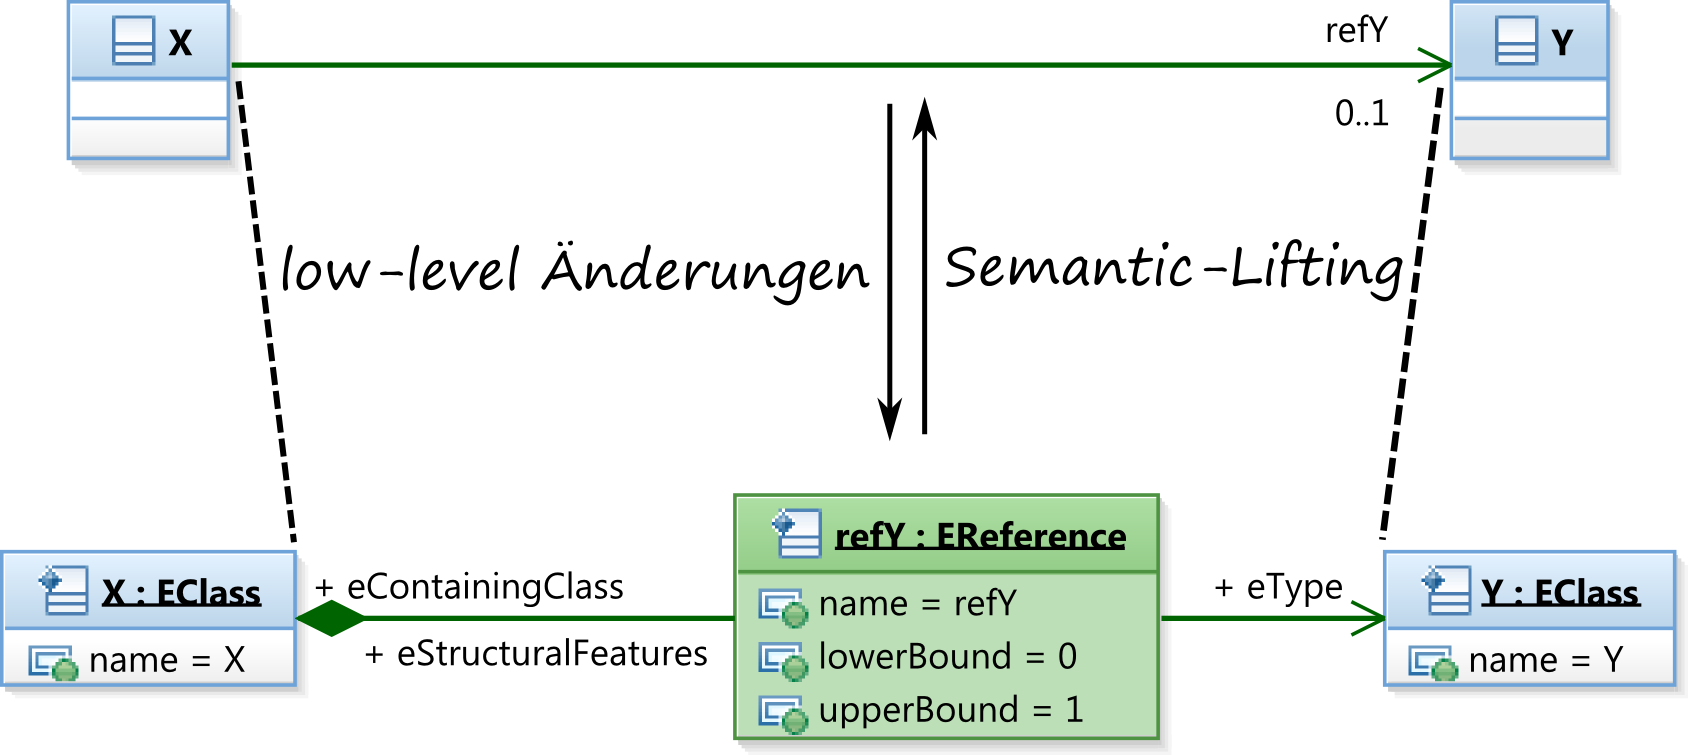
\includegraphics[width=1.0\textwidth]{images/semantic_lifting.png}
  \caption{Semantic-Lifting}
  \label{fig:semantic_lifting}
\end{figure}

Abbildung \ref{fig:semantic_lifting} demonstriert dies anhand des Einfügens einer Referenz zwischen
zwei Klassen eines Ecore Modells (Abbildung \ref{fig:ecore_metamodel}). Wie man sieht wird dazu in
der internen Darstellung eine neue Klasse angelegt, die diese Referenz repräsentiert. Sowohl der
Name als auch die Multiplizitäten der Referenzen werden als Attribute in dieser Klasse gespeichert.
Zusätzlich werden noch mehrere Referenzen benötigt, welche Quelle und Ziel der eingefügten Referenz
festlegen. Eben diese s.g. \textbf{low-level Änderungen} werden durch das Differenzwerkzeug erkannt
und angezeigt. Die Frage ist nun, ob es möglich ist nur anhand der low-level Änderungen zu erkennen,
welche Editieroperation auf das Modell angewendet wurde, um dem Benutzer so eine Differenz auf Basis
der externen Repräsentation anzuzeigen.

Das Konzept "`A Rule-Based Approach to the Semantic Lifting of Model Differences in the Context of
Model Versioning"' \cite{KeKT2011ASE} beschäftigt sich mit genau dieser Problematik. Hier wird ein
Algorithmus beschrieben, der einer beliebigen Anzahl von low-level Änderungen wieder die
entsprechenden Editieroperationen zuordnen kann. Dazu werden Editierregeln verwendet, welche eine
Editieroperation beschreiben. Die Editierregeln werden dann dazu benutzt, um das der Editieroperation
entsprechende Muster von low-level Änderungen wieder zu erkennen.  Dieser Prozess wird in Anlehnung
an das Konzept im Folgenden als \textbf{Semantic-Lifting} bezeichnet. 

Diese Arbeit beschreibt die praktische Untersuchung, Implementierung und die daraus resultierenden
Ergebnisse des Semantic-Liftings. Dazu werden in Kapitel \ref{grundlagen} zunächst die wichtigsten
Technologien für dieses Projekt besprochen. Kapitel \ref{diffPipe} gibt einen Überblick über
den im Folgenden beschriebenen Algorithmus. Hierzu wird in den Kapiteln \ref{editierregeln},
\ref{generierung} und \ref{verwaltung} die Erstellung von Editierregeln und die Generierung von
daraus resultierenden Mustern zur Erkennung der Editeroperationen erläutert. In den Kapiteln
\ref{resource_sets}, \ref{recognition}, \ref{post_processing}, \ref{sequential} und
\ref{benutzer}, wird dann dargelegt, wie mit Hilfe dieser Erkennungsmuster, das eigentlich
Semantic-Lifting durchgeführt wird. In Kapitel \ref{evaluierung} und \ref{schlussfolgerung} werden
zum Schluss die Ergebnisse des Semantic-Liftings ausgewertet.
